\documentclass[11pt, fleqn]{article}

\documentclass[11pt, fleqn]{article}

\usepackage[usenames,dvipsnames,svgnames,table]{xcolor}
\usepackage{amsmath}
\usepackage{amsfonts}
\usepackage[margin=1in]{geometry} % To set the margin widths
\usepackage{graphicx}
\usepackage{listings}
\usepackage{multirow}
\usepackage{tabularx}
\usepackage{varioref}
\usepackage[noabbrev,capitalize]{cleveref}
\usepackage[group-separator={,}]{siunitx}
\usepackage{subcaption}
\usepackage{titlesec}
\usepackage{lscape}
\usepackage{bm}
\usepackage[titletoc,toc,title]{appendix}

\lstset{
  frame=single,
  basicstyle=\ttfamily,% print whole listing small
  language=R,
  aboveskip=3mm,
  belowskip=3mm,
  showstringspaces=false,
  columns=flexible,
  numbers=none,
  commentstyle=\color{ForestGreen},
  stringstyle=\color{Maroon},
  breaklines=true,
  breakatwhitespace=true,
  tabsize=2,
  literate={<-}{{$\gets$}}1 {~}{{$\sim$}}1
}

\sisetup{output-exponent-marker=\textsc{e}}

\setlength{\parskip}{12pt} % Sets a blank line in between paragraphs
\setlength\parindent{0pt} % Sets the indent for each paragraph to zero

% \crefname{figure}{Figure}{Figures}
% \crefname{section}{Section}{Sections}
% \crefname{table}{Table}{Tables}
% \crefname{lstlisting}{Listing}{Listings}

\setlength{\parskip}{12pt} % Sets a blank line in between paragraphs
\setlength\parindent{0pt} % Sets the indent for each paragraph to zero

\begin{document}

\title{Machine Learning (41204-01)\\HW \#4}
\author{Will Clark $\vert$ Matthew DeLio \\
\texttt{will.clark@chicagobooth.edu} $\vert$ \texttt{mdelio@chicagobooth.edu} \\
University of Chicago Booth School of Business}
\date{\today}
\maketitle

\section{Cleaning and Partitioning the Dataset}
The dataset available to us has been highly anonymized and not really interpretable in any human-readable form.  They only provide numbers and factors that we can feed into our model to predict some event (in our case customer ``churn'').  After choosing to predict ``churn'' we took our dataset and went about cleaning it up.  To do this we employ the suggested algorithm contained in the assignment:
\begin{itemize}
\item Remove covariates containing all NAs.  This brings the number of covariates from 230 to 211\footnote{We considered using a lower threshold here, but were concerned about arbitrarily throwing out interesting covariates.  Instead we chose to let the variable selection algorithms perform their task of removing them if they contained no useful data.};
\item Replace remaining NAs of a covariate with its sample mean;
\item Using the relative frequency of levels to collapse and merge factors together using the following rules\footnote{This was applied only to covariates with $>50$ factor levels.}:
\begin{itemize}
\item Levels with $<0.5\%$ (n=$<250$) of observations are set to ``low''
\item Levels with $0.5-1.0\%$ (n=250 to 500) of observations are set to ``medium''
\item Levels with $1.0-2.0\%$ (n=500 to 1,000) of observations are set to ``high''
\item Levels with $>2.0\%$ of observations are left as is.
\end{itemize}
\end{itemize}

Prior to performing variable selection, we partition our dataset up into 3 pieces holding 60\% in the training set and 20\% each in the validation and test sets.  The elements are chosen randomly, without replacement, from the cleaned dataset\footnote{We realize that, ideally, we would clean only the training data, applying the same transformations to the validation and test set, but this proves to be too intractable for the homework.}.

\section{Variable Selection}
\subsection{Initial Work}
Our initial work revolved mainly around building a random forest implementation due for both the variable selection and final model (see \cref{sec:init_rf,sec:mod_rf} for subsequent, but similar work) because of the simplicity of getting it working.  After completing this work we noticed that model chose to largely ignore the rare event in aggregate, which while maximising the precision of the overall algorithm lead to 100\% mis-prediction for True Positives.  

To address this issue we employed an oversampling technique where we take the partitioned training data and even out the occurrence of positive and negative outcomes such that the 7.3\% of positive outcomes becomes 50\%.  This results in the reduction in the number of training samples from 30,000 to 4,438.

The subsequent sections (unless otherwise noted) use this oversampled training data to create a fitted model.

\subsection{Random Forest}\label{sec:init_rf}
This tool uses a random forest to fit a relatively small number of tree (500) to our oversampled dataset.  After training this model we use the random forest's variable importance output to determine which of the variables are most important.  See \cref{fig:rf_var_sel} for a graphical representation of this list.  Note that the plot shows the mean decrease in accuracy that would result if the given variable is removed from the model.  Using this ranking we select the 30 more important covariates to fit later in \cref{sec:mod_rf}.

\begin{figure}[!htb]
  \centering
  \caption{Random Forest Important Variables}
  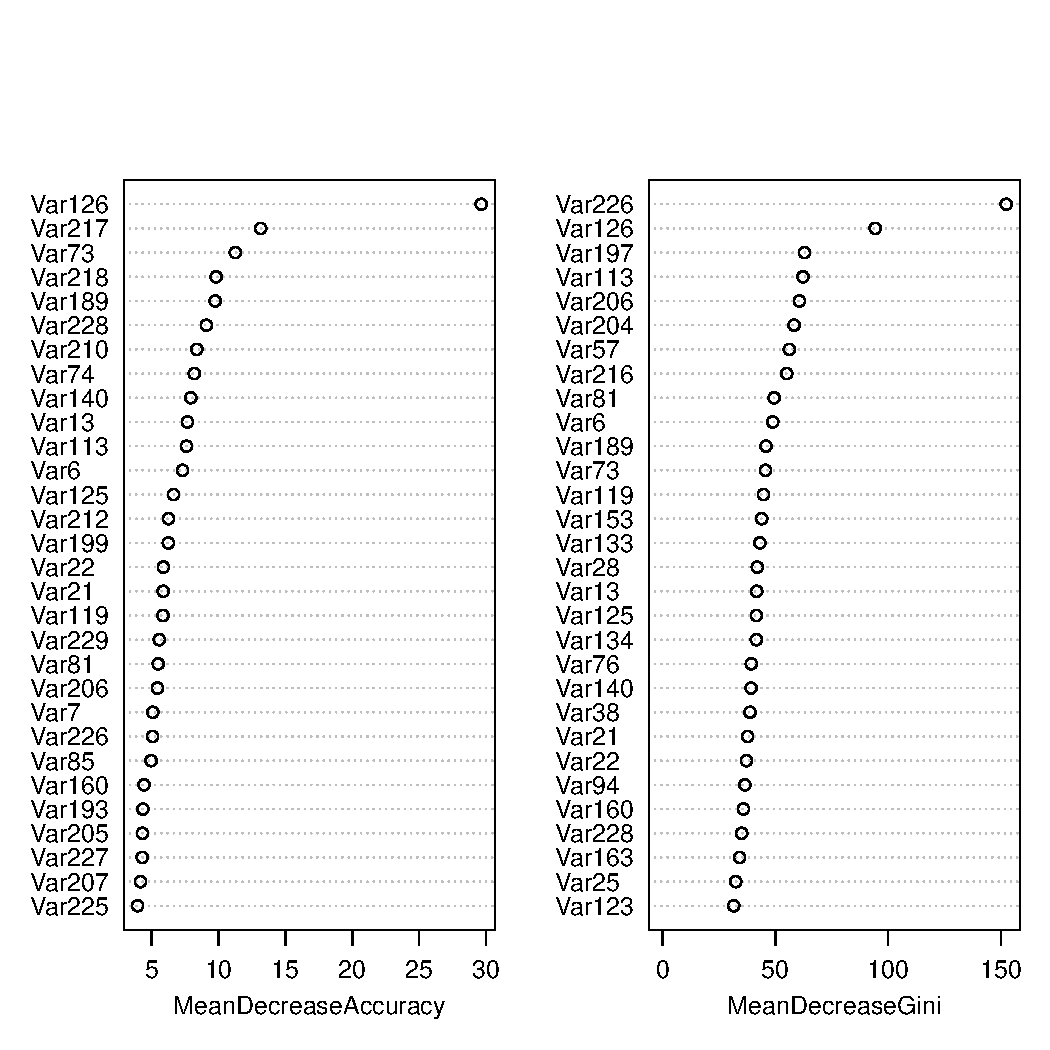
\includegraphics[scale=.5]{rf_var_sel.pdf}
  \label{fig:rf_var_sel}
\end{figure}


\subsection{The Gamma-Lasso}

Another tool for variable reduction is regression with $L_1$ regularization (i.e. the lasso). The process of estimating a model while penalizing non-zero coefficients is an algorithmic way to reduce the dimensionality of our data set. There are two ways we can add to the dimension reduction process:
\begin{enumerate}
\item Using the Gamma-Lasso in the package \texttt{gamlr} allows us to control the concavity of the penalty function. A more concave penalty function increases the number of variables held out of the model and reduces dimensionality even further.
\item The Gamma-Lasso algorithm gives us a series of models to choose from, each corresponding to a penalty tuning parameter $\lambda$. We can choose $\lambda$ (which determines the variables excluded from the model) according to different information criteria: the Akaike information criterion, the corrected Akaike information criterion, or the Bayes information criterion. In general, the BIC will give us the simplest model (i.e. reduce dimensionality the most), so we will use this criterion to select a model and a set of variables.
\end{enumerate}
By setting $\lambda=10$ (which is a very high concavity tuning parameter) and selecting a model based on the BIC, the Gamma-Lasso chooses a model with only 11 variables.

\subsection{Principal Components Analysis (PCA)}

Another dimension reduction tool is principal components analysis. Here, the goal is to transform our data set into a collection of orthogonal vectors (i.e. principal components). We can order the vectors by the amount of variation in our dependent data that they explain, and choose the first $N$ principal components to represent the data.

The purpose is to reduce the dimensionality of our original data set into a small number of series that together explain a large share of the variation in our dependent variable. There is no obvious way to choose how many principal components to include. We would need to include 53 principal components to capture half of the observed variation in the data. We would need to include only 13, however, to capture one quarter of the observed variation in the data. For the rest of this exercise, we will proceed using the first 13 principal components. This allows us to capture 25 percent of the variation in the data while dropping almost 95 percent of the data series (not even including the series that were dropped as part of the data cleaning process). 

\section{Model Selection}

\subsection{Logistic Regression}
The first predictive model we will try is a basic logistic regression model. We will use each of our three sets of reduced variables described above (from the random forest variable importance, the Gamma-Lasso, and PCA). We will simply estimate a linear model and see how well it predicts  churn out of sample.



\subsection{Random Forest}\label{sec:mod_rf}
Using only the covariates identified in \cref{sec:init_rf} we fit a much larger number of trees to our dataset.  The resulting model is then used to fit the non-oversampled validation set which results in the confusion matrix shown below.  Note that with this algorithm we have achieved a fairly decent sensitivity of 75\% (true-positive detection rate) at the expense of a relatively low specificity of just 58\% (i.e. we have many false-positives).

\begin{verbatim}
Confusion Matrix and Statistics

          Reference
Prediction TRUE FALSE
     TRUE   568  3891
     FALSE  193  5348
                                          
               Accuracy : 0.5916          
                 95% CI : (0.5819, 0.6013)
    No Information Rate : 0.9239          
    P-Value [Acc > NIR] : 1               
                                          
                  Kappa : 0.1007          
 Mcnemar's Test P-Value : <2e-16          
                                          
            Sensitivity : 0.7464          
            Specificity : 0.5789          
         Pos Pred Value : 0.1274          
         Neg Pred Value : 0.9652          
             Prevalence : 0.0761          
         Detection Rate : 0.0568          
   Detection Prevalence : 0.4459          
      Balanced Accuracy : 0.6626          
                                          
       'Positive' Class : TRUE
\end{verbatim}

\subsection{Boosting}
Another possible predictive model is regression tree boosting using the packages \texttt{gbm} and \texttt{caret}. We have three different training data sets available: the data selected by the random forest, the data selected by the Gamma-Lasso, or the principal components discussed above. For each set of training data, we also have the opportunity to tune our boosting tree with the interaction depth, number of trees, and the shrinkage parameter.

To tune the boosting tree algorithm, we use the \texttt{caret} package to perform 5-fold cross-validation on each combination of parameters. We consider values of interaction depth of 1, 5, and 9; we try using 500, 1000, and 1500 trees; and we use shrinkage parameters of 0.01, 0.05, and 0.10. All told, there are 27 different combinations of tuning parameters, for each of three different sets of input variables (depending on the dimension reduction strategy we used). 

In \cref{tab:boost_tune} we can see the results of this tuning exercise. For each dimension reduction strategy, we show the optimal set of tuning parameters as well as the out-of-sample accuracy (on a validation data set not used to train the model). We can see that the boosting tree trained on data selected by the Gamma-Lasso is the best (with 67 percent accuracy), followed closely by the variables selected by the random forest (with 65 percent accuracy). The principal components do not fare well, producing out-of-sample accuracy of only 55 percent.

% latex table generated in R 3.2.2 by xtable 1.7-4 package
% Thu Oct 22 06:15:56 2015
\begin{table}[ht]
\centering
\caption{Optimal Tuning Parameters for Boosting Tree} 
\label{tab:boost_tune}
\begin{tabular}{rrrrr}
  \hline
Dimension Reduction & Number of Trees & Interaction Depth & Shrinkage & Accuracy \\ 
  \hline
Random Forest & 500 &   5 & 0.01 & 0.65 \\ 
  Gamma-Lasso & 1000 &   5 & 0.01 & 0.67 \\ 
  PCA & 1000 &   1 & 0.01 & 0.55 \\ 
   \hline
\end{tabular}
\end{table}


\subsection{Summary}


\section{Out-of-Sample Prediction}
% In case we want to present all of these.
To perform out-of-sample prediction we use the last, heretofore unused, piece of our data initial data, the test-set.  Below we present the out-of-sample statistics for the best of the algorithms we explored earlier.

% Feel Free to yank this section if it doesn't make sense, just didn't want you to have to write this up.
Below is the out-of-sample confusion matrix/statistics for the covariates chosen by and a model generated from a random-forest (i.e. the one developed in \cref{sec:mod_rf}).  As expected the confusion matrix remains largely unchanged from the one estimated by the validation sample.  The accuracy remains in the 95\% CI prescribed earlier, and sensitivity and specificity remain within a percentage of their respective values.  The overall issue with this model is its rather low specificity, which leads us to prefer other models over it if they can perform better in these two dimensions.

\begin{verbatim}
Confusion Matrix and Statistics

          Reference
Prediction TRUE FALSE
     TRUE   509  3998
     FALSE  183  5310
                                          
               Accuracy : 0.5819          
                 95% CI : (0.5722, 0.5916)
    No Information Rate : 0.9308          
    P-Value [Acc > NIR] : 1               
                                          
                  Kappa : 0.0862          
 Mcnemar's Test P-Value : <2e-16          
                                          
            Sensitivity : 0.7355          
            Specificity : 0.5705          
         Pos Pred Value : 0.1129          
         Neg Pred Value : 0.9667          
             Prevalence : 0.0692          
         Detection Rate : 0.0509          
   Detection Prevalence : 0.4507          
      Balanced Accuracy : 0.6530          
                                          
       'Positive' Class : TRUE
\end{verbatim}

\end{document}

% \input{.tex}

% \begin{figure}
%   \centering
%   \begin{subfigure}[b]{0.49\textwidth}
%     \caption{}
%     \includegraphics[width=\textwidth]{.pdf}
%     \label{fig:}
%   \end{subfigure}
%   \hfill
%   \begin{subfigure}[b]{0.49\textwidth}
%     \caption{}
%     \includegraphics[width=\textwidth]{.pdf}
%     \label{fig:}
%   \end{subfigure}
%   \caption{}
% \end{figure}

% \begin{figure}[!htb]
%   \centering
%   \caption{}
%   \includegraphics[scale=.5]{.pdf}
%   \label{fig:}
% \end{figure}

